\chapter{Analyse des Wearable-Marktes}
\section{Überblick}
	\begin{itemize}
		\item verschiedene OS
			\begin{itemize}
				\item Android Wear
				\item WebOS
			\end{itemize}
		\item Vor-/Nachteile OS'
			\begin{itemize}
				\item z.B. sowohl mit AndroidWear als auch mit iOS nutzbar
			\end{itemize}
	\end{itemize}

\subsection{Marktanteile Anbieter}
\begin{figure}[h!]
	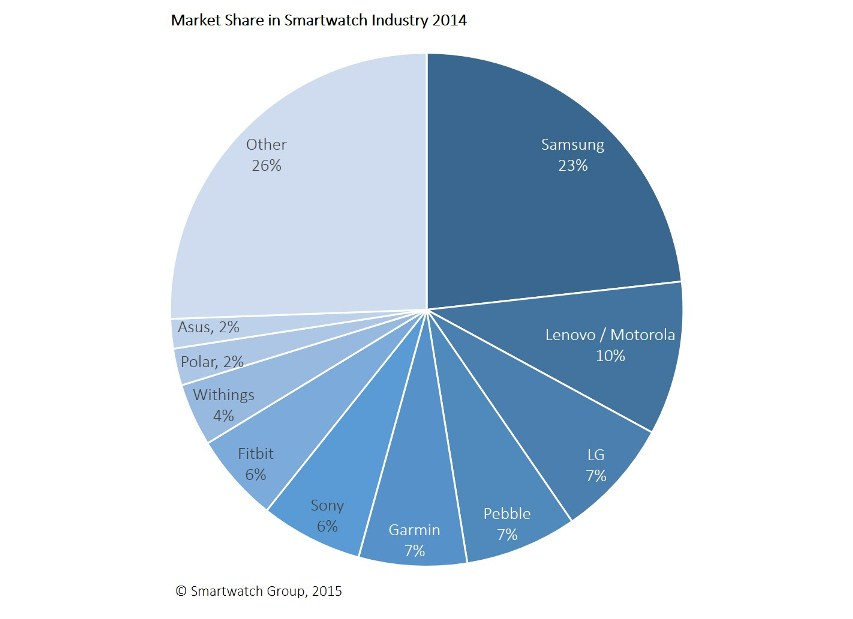
\includegraphics{Bilder/Market_Share_Smartwatch_Companies_2014}
	%\captionsetup{width=0.6\textwidth}	
	\caption[Marktanteile Smartwatch-Anbieter 2014]{Marktanteile Smartwatch-Anbieter 2014\\\hspace{\textwidth}(Quelle: http://www.smartwatchgroup.com)}
\end{figure}

\section{Prognose}
\section{Fitnesstracker}
\subsection{Definition}
Ein Fitness Tracker, auch Fitness-Armband, Smart Band oder Activity Tracker, ist ein Gerät oder eine Applikation zur Aufzeichnung und Versendung Fitness-relevanter Daten wie etwa Laufstrecken, Kalorienverbrauch und in manchen Fällen auch Herzschlagfrequenz oder Schlafqualität. Die Bezeichnung wird hauptsächlich für am Körper tragbare elektronische Überwachungsgeräte verwendet, welche, in vielen Fällen drahtlos, mit einem Computer oder Smartphone für die Datenerfassung über einen längeren Zeitraum synchronisiert werden. Abgesehen von diesen tragbaren Geräten, gibt es auch vergleichbare Applikationen für Smartphones und Facebook.\footnote{Quelle: \url{http://de.wikipedia.org/wiki/Activity\_Tracker}, Stand: 25.03.2015}

\subsection{Aktuelle Beispielgeräte}
\begin{longtable}{p{4cm}p{4cm}p{4cm}p{4cm}}

	% 1. line
	  \rule{0pt}{120pt}
	  \rotatebox{90}{Samsumg Gear Fit} 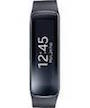
\includegraphics{Bilder/FitnessTracker/samsung_gear_fit}
	& \rotatebox{90}{Garmin Vivosmart} 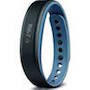
\includegraphics{Bilder/FitnessTracker/garmin_vivosmart}
	& \rotatebox{90}{Fitbit Charge HR} 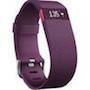
\includegraphics{Bilder/FitnessTracker/fitbit_charge_hr}
	& \rotatebox{90}{LG Lifeband Touch} 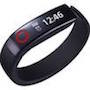
\includegraphics{Bilder/FitnessTracker/lg_lifeband_touch}\\
    % 2. line
      \rule{0pt}{120pt}
      \rotatebox{90}{Runtastic Orbit} 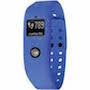
\includegraphics{Bilder/FitnessTracker/runtastic_orbit}
	& \rotatebox{90}{Withings Activité} 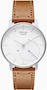
\includegraphics{Bilder/FitnessTracker/withings_activite}
	& \rotatebox{90}{Huawei TalkBand} 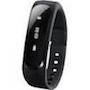
\includegraphics{Bilder/FitnessTracker/huawei_talkband}
	& \rotatebox{90}{Sony SmartBand Talk} 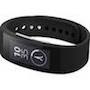
\includegraphics{Bilder/FitnessTracker/sony_smartband_talk}\\
\end{longtable}

\newpage

\section{Smartwatches}
\subsection{Definition}
Eine Smartwatch (englisch für schlaue Uhr) ist eine Armbanduhr, die zusätzlich über Sensoren, Aktuatoren (z. B. Vibrationsmotor) sowie zusätzliche Computerfunktionalität und -konnektivität verfügt. Aktuelle Smartwatches können neben der Uhrzeit weitere Informationen darstellen und lassen sich meist über zusätzliche Programme (sogenannte Apps) vom Anwender individuell mit neuen Funktionen aufrüsten.\footnote{Quelle: \url{http://de.wikipedia.org/wiki/Smartwatch}, Stand: 25.03.2015}
\newpage

% --- Vergleich Features ---
\begin{landscape}
\subsubsection{Vergleich Features}
\renewcommand{\arraystretch}{1.5}
% --- Vergleich Features, Teil 1 ---
\begin{longtable}{p{2.8cm}p{3.5cm}p{3.5cm}p{3.5cm}p{3.5cm}p{3.5cm}}

	% Header
	& \rotatebox{90}{LG G Watch} 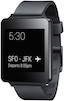
\includegraphics{Bilder/SmartWatch/lg_g_watch}
	& \rotatebox{90}{LG G Watch R} 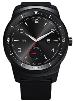
\includegraphics{Bilder/SmartWatch/lg_g_watch_r}
	& \rotatebox{90}{LG Watch Urbane LTE} 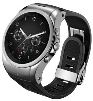
\includegraphics{Bilder/SmartWatch/lg_watch_urbane_lte}
	& \rotatebox{90}{Motorola Moto 360} 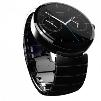
\includegraphics{Bilder/SmartWatch/moto_360}
	& \rotatebox{90}{Apple Watch} 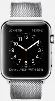
\includegraphics{Bilder/SmartWatch/apple_watch}\\
	\hline
	\endfirsthead
	
	\multicolumn{3}{l}{Fortsetzung} \\
	& {LG G Watch}
	& {LG G Watch R}
	& {LG Watch Urbane LTE}
	& {Motorola Moto 360}
	& {Apple Watch} \\
	\hline
	\endhead

	% Content
	Display
		& 1.65 Zoll \newline
			280x280px (204ppi) \newline
			IPS
		& 1.3 Zoll \newline
			320x320px (245ppi) \newline
			P-OLED
		& 1.3 Zoll \newline
			320x320px (245ppi) \newline
			P-OLED
		& 1.56 Zoll \newline
			320x290 (205ppi) \newline
			IPS
		& 1.32 Zoll \newline
			272x340 \\
	Prozessor
		& 1,2-GHz \newline Snapdragon 400
		& 1,2-GHz \newline Snapdragon 400
		& 1,2-GHz \newline Snapdragon 400
		& 1-GHz \newline Texas Instrument\newline OMAP 3
		& Apple S1 (SIP)\newline System in a package \\
	RAM
		& 512 MB
		& 512 MB
		& 1 GB
		& 512 MB
		& SIP\\
	interner Speicher
		& 4 GB
		& 4 GB
		& 4 GB
		& 4 GB
		& 8 GB \\
	Akku
		& 400 mAh
		& 410 mAh
		& 700 mAh
		& 320 mAh
		& ab 205 mAh\\
	Betriebssystem
		& Android Wear
		& Android Wear
		& LG Wear Platform \newline (ehem. HP WebOS)
		& Android Wear
		& Watch OS \\
	Kompatibilität
		& Android 4.3+
		& Android 4.3+
		& Autonom
		& Android 4.3+
		& iOS 8+\\
	Netzwerk
		& -
		& -
		& LTE
		& - 
		& -\\
	Verbindung
		& BLE 4.0
		& BLE 4.0
		& BLE 4.0 \newline
			Wifi 802.11 b/g/n \newline
			NFC
		& BLE 4.0 \newline
			WiFi
		& BLE 4.0 \newline
			WiFi 802.11 b/g/n \newline
			NFC \\
	Schnittstellen
		& Mikrofon
		& Mikrofon
		& Mikrofon \newline
			Lautsprecher
		& Mikrofon
		& Mikrofon \newline
			Lautsprecher \\
	Sensoren
		& Beschleunigungssensor \newline
			Gyroskop \newline
			Kompass \newline
			Schrittzähler
		& Herzfrequenz \newline
        		Beschleunigungssensor \newline
			Gyroskop \newline
			Kompass \newline
			Schrittzähler
		& Herzfrequenz \newline
        		Beschleunigungssensor \newline
			Gyroskop \newline
			Kompass \newline
			Schrittzähler \newline
			Luftdrucksensor
		& Herzfrequenz \newline
		    Beschleunigungssensor \newline
			Gyroskop \newline
			Kompass \newline
			Schrittzähler
		& Beschleunigung \newline
			GPS \newline
			Gyrometer \newline
			Herzfrequenz \newline
			Kompass \newline
			Multi \& ForceTouch \newline
			Schrittzähler \\
	Sonstiges
		& IP67 \newline
			Always-On Display
		& IP67
		& IP67
		& IP67
		& spritzwassergeschützt \\
	Abmessung
		& 37.9 x 45.6 x 9.95 mm
		& 46.4 x 53.6 x 11.1 mm
		& 46 x 52 x 10.9 mm
		& 46 x 46 x 11.5 mm
		& 38.6 x 33.3 x 10.5 mm \newline
		42 x 35.9 x 10.5 mm\\
	Gewicht
		& 63g
		& 62g
		& 45 - 115g
		& 49 - 124g
		& ab 73g\\ 
	Markteinführung
		& Jun 2014
		& Nov 2014
		& na 
		& Sep 2014
		& Apr 2015\\
	Preis\footnote{Preise von digitec.ch (günstigstes Modell), Stand: 17.03.2015 oder neuer}
		& CHF 99.00
		& CHF 199.00
		& na
		& CHF 199.00
		& ab CHF 389.00 \\
	\hline
	\caption{Vergleich Features von Smartwatches, Teil 1} \\
\end{longtable}
\newpage

% --- Vergleich Features, Teil 2 ---
\begin{longtable}{p{2.8cm}p{3.5cm}p{3.5cm}p{3.5cm}p{3.5cm}p{3.5cm}}

	% Header
	& \rotatebox{90}{Huawei Watch} 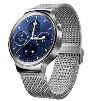
\includegraphics{Bilder/SmartWatch/huawei_watch}
	& \rotatebox{90}{Sony SmartWatch 3} 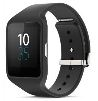
\includegraphics{Bilder/SmartWatch/sony_smartwatch_3}
	& \rotatebox{90}{Samsung Gear S} 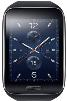
\includegraphics{Bilder/SmartWatch/samsung_gear_s}
	& \rotatebox{90}{Samsung Gear Live} 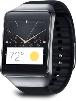
\includegraphics{Bilder/SmartWatch/samsung_gear_live}
	& \rotatebox{90}{Asus ZenWatch} 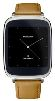
\includegraphics{Bilder/SmartWatch/asus_zen_watch} \\
	\hline
	\endfirsthead
	
	\multicolumn{3}{l}{Fortsetzung} \\
	& {Huawei Watch}
	& {Sony SmartWatch 3}
	& {Samsung Gear S}
	& {Samsung Gear Live}
	& {Asus ZenWatch} \\
	\hline
	\endhead	

	% Content
	Display
		& 1.4 Zoll \newline
			400x400 (286ppi) \newline
			AMOLED
		& 1.6 Zoll \newline
			320x320px
		& 2 Zoll \newline
			480x360px (300ppi) \newline
			Super AMOLED
		& 1.63 Zoll \newline
			320x320px (278ppi) \newline
			Super AMOLED
		& \newline
			320x320px (278ppi) \newline
			AMOLED \\
	Prozessor
		& 1.2 GHz \newline
			Snapdragon 400
		& na
		& na
		& na
		& \\
	RAM
		& 512 MB
		& 512 MB
		& 512 MB
		&
		& 512 MB\\
	interner Speicher
		& 4 GB
		& 4 GB
		& 4 GB
		& 4 GB
		& 4 GB\\
	Akku
		& 300 mAh
		& 420 mAh 
		& 300 mAh
		& 300 mAh
		& 369 mAh\\
	Betriebssystem
		& Android Wear
		& Android Wear
		& Tizen 
		& Android Wear
		& Android Wear \\
	Kompatibilität
		& Android 4.3+
		& Android 4.3+
		& Android 4.3+
		& Android 4.3+
		& Android 4.3+ \\
	Netzwerk
		& -
		& -
		& 3G
		& -
		& -\\
	Verbindung
		& BLE 4.0
		& BLE 4.0 \newline
			NFC
		& BLE 4.0
		& BLE 4.0
		& BLE 4.0\\
	Schnittstellen
		& Mikrofon
		& Mikrofon \newline
			Lautsprecher
		& Mikrofon
		& Mikrofon
		& Mikrofon \\
	Sensoren
		& Beschleunigungssensor \newline
			Gyrometer \newline
			Herzfrequenz \newline
			Schrittzähler
		& Beschleunigungssensor \newline
			Gyrometer \newline
			Kompass \newline
			GPS
		& Beschleunigungssensor \newline
			GPS \newline
			Gyrometer \newline
			Helligkeitssensor\newline			
			(Multi-)Touch
		& Beschleunigungssensor \newline
			Gyrometer \newline
			Herzfrequenz \newline
			(Multi-)Touch \newline
			Schrittzähler 
		& Beschleunigungssensor \newline
			Gyrometer \newline
			Kompass \newline
			GPS\\
	Sonstiges
		& IP67
		& IP68
		& IP67 \newline
			Kopfhörerbuchse
		&
		& IP55\\
	Abmessung
	    & 42 x 42 x 11.3 mm
		& 46.4 x 53.6 x 11.1 mm
		& 46 x 52 x 10.9 mm
		& 46 x 46 x 11.5 mm
		& 42 x 35.9 x 10.5 mm\\
	Gewicht
		& na
		& 45g
		& na
		& 59g
		& 75g\\ 
	Markteinführung
		\\
	Preis\footnote{Preise von digitec.ch (günstigstes Modell), Stand: 17.03.2015 oder neuer}
		& CHF 349.00	
		& CHF 229.00
		& CHF 329.00
		& -
		& CHF 249.00\\
	\hline
	\caption{Vergleich Features von Smartwatches, Teil 2} \\
	
\end{longtable}
\end{landscape}

\section{Andere Wearables}
http://www.digitsole.com/

\section{Verfügbare Apps/Frameworks}
http://die-smartwatch.de/android-wear-apps\#musthave\\
http://die-smartwatch.de/2015/03/15/umwelt-computer-per-android-wear-und-pebble-sperren.html\\
http://www.kiwimotion.io/